\documentclass[10pt, a4paper]{article}
\usepackage[paper=a4paper, left=1.5cm, right=1.5cm, bottom=1.5cm, top=3.5cm]{geometry}
\usepackage[T1]{fontenc}
\usepackage[spanish]{babel}
\usepackage[utf8]{inputenc}
\usepackage{indentfirst}
\usepackage{fancyhdr}
\usepackage{a4wide}
\usepackage[dvipsnames,usenames]{color}
\usepackage{float}
\usepackage{amsmath}
\usepackage{epsfig}
\usepackage{listings}
\usepackage{listingsutf8}
\usepackage{graphicx}
\usepackage{amsfonts}
\usepackage{verbatim}
\usepackage{fixltx2e}
\usepackage{latexsym}
\usepackage{algpseudocode}
\usepackage[section]{algorithm}
\usepackage{lastpage}
\usepackage[colorlinks=true, linkcolor=blue]{hyperref}
\usepackage{calc}

\newcommand{\f}[1]{\text{#1}}
\newcommand{\real}{\mathbb{R}}
\newcommand{\nat}{\mathbb{N}}
\newcommand{\eme}{\mathcal{M}}
\newcommand{\emeh}{\widehat{\mathcal{M}}}
\newcommand{\ere}{\mathcal{R}}

\sloppy

\setlength{\voffset}{-0.5cm}
\setlength{\hoffset}{0.7cm}
\setlength{\headsep}{0pt}
\setlength{\headheight}{0pt}
\setlength{\oddsidemargin}{-0.7in}
\setlength{\marginparwidth}{-0.5cm}
\setlength{\textwidth}{18cm}
\setlength{\footskip}{2pt}
\setlength{\topmargin}{0in}
\setlength{\textheight}{25cm}
\setlength{\fboxrule}{3pt}

\begin{document}
\thispagestyle{empty}
\begin{center}

\Huge{ \bf{UNIVERSIDAD DE BUENOS AIRES}}
\\
\LARGE{\bf{Facultad de Ciencias Exactas y Naturales}}
\\
\textbf{Departamento de Computaci\'on}
\\
\textbf{M\'etodos Num\'ericos}
\vspace{2.0\baselineskip}
\end{center}


\begin{figure}[h] %[h] Aqui [b] para button [t] para top
\begin{center}

\includegraphics[width=100pt]{./image.jpeg}
\end{center}
\end{figure}
\begin{center}
\vspace*{0.7cm}

\huge{\bf TRABAJO PR\'ACTICO N\'UMERO 3}\\
\huge{Reconocimiento óptico de caracteres.}
\vspace*{2cm}

\end{center}

\LARGE {\textbf{Alumnos:}}\\
\Large{\textsl{Izcovich, Sabrina} $|$ sizcovich@gmail.com}\\
\Large{\textsl{Otero, Fernando} \hspace{0.1cm}$|$ fergabot@gmail.com}\\
\Large{\textsl{Vita, Sebasti\'an} \hspace{0.37cm}$|$ sebastian\_vita@yahoo.com.ar}
\vspace{0.6cm}

\LARGE {\textbf{Palabras Clave:}}\\
\large {OCR - Método de Potencia - SVD - QR}
\vspace*{0.7cm}

\LARGE{\textbf{Resumen:}}\\
\large{Este trabajo consiste en un análisis sobre la implementación de un método de reconocimiento de dígitos manuscritos basado en la descomposición en valores singulares. Dicha implementación consiste en un programa encargado de leer imágenes que, a partir de la descomposición en valores singulares, logra determinar de qué dígito se trata. Para que las pruebas fueran posibles, utilizamos la base de datos MNIST que nos proporcionó una gran cantidad de imágenes de cada dígito que luego serían comparadas con el dígito a definir. Para alcanzar nuestro objetivo debíamos hallar los autovalores y autovectores de la matriz de covarianza de la base de datos. Para ello, utilizamos, en primer lugar, el Método de Potencia y, debido a que éste generaba complicaciones, optamos por QR. El estudio realizado se focalizó en los parámetros elegidos para aplicar el método que resultaron determinantes a la hora de hallar efectividad del mismo.}
\newline
 
\newpage
%Pagina de titulo e indice
\thispagestyle{empty}

\tableofcontents

\newpage

\section{Introducci\'on te\'orica}
Para la realización del estudio de señales, utilizamos los siguientes conceptos:
\begin{itemize}
\item {\textbf{Reconocimiento óptico de caracteres:}} Es un proceso dirigido a la digitalización de textos. Dicho proceso consiste en identificar automáticamente símbolos o caracteres pertenecientes a un determinado alfabeto a partir de una imagen. Existen OCR muy diversos según los tipos de problemas que abordan y las funcionalidades que ofrecen: para designar el reconocimiento de caracteres manuscritos se utiliza el ICR (intelligent character recognition), para la verificación de contenidos previamente conocidos se utiliza OCV (optical character verification) y, por último, para el reconocimiento de marcas se utiliza OMR (optical mark recognition). Nuestro trabajo estará implícitamente enfocado en el ICR. 
\item {\textbf{Covarianza:}} Consiste en una medida de dispersión conjunta a un par de variables. En otras palabras, es el dato básico para determinar si existe una dependencia entre ambas variables y, además, es el dato necesario para estimar otros parámetros básicos, como el coeficiente de correlación lineal o la recta de regresión. Se encuentra representada de la siguiente manera: $$cov(X, Y) = \frac{\sum_{i=1}^{n} (x_i - \bar{X})(y_i - \bar{Y})}{n}$$
\item {\textbf{MNIST:}} Consiste en una base de datos de dígitos manuscritos. Dichos dígitos tienen un tamaño normalizado y se encuentran centrados en una imagen de tamaño fijo. Es utilizada para aprender técnicas y patrones de reconocimiento de datos del mundo real. En nuestro caso, utilizamos las imágenes y las etiquetas para evaluar nuestro código y lograr la obtención de resultados.
\item {\textbf{Método de Potencia:}} Consiste en una técnica iterativa que permite determinar el valor característico dominante de una matriz, es decir, el valor característico con mayor magnitud. Dicho método es utilizado para hallar tanto autovalores como autovectores. Para aplicarlo, supusimos que la matriz $A$ de $n$x$n$ tiene $n$ valores característicos $\lambda_{1}$, $\lambda_{2}$,...,$\lambda_{n}$ con un conjunto asociado de vectores característicos linealmente independientes ${v_{1}, v_{2},...,v_{n}}$. Más aún, supusimos que $A$ tiene exactamente un valor característico, $\lambda_{1}$, cuya magnitud es la mayor, por lo que $|\lambda_{1}| > |\lambda_{2}| \geq |\lambda_{3}| \geq ... \geq |\lambda_{n}| \geq 0$.
\item {\textbf{Factorización QR:}} Consiste en una factorización matricial siguiendo la siguiente propiedad: Para toda matriz A de tamaño mxn cuyas columnas forman un conjunto linealmente independiente, existe una matriz Q de tamaño mxn, cuyas columnas forman un conjunto ortonormal y una matriz triangular superior R de tamaño nxn tales que A = QR.
\item {\textbf{Descomposición en valores singulares:}} Siendo uno de los más grandes desarrollos aportados por el álgebra lineal moderna con importantes aplicaciones en diversos campos, la descomposición en valores singulares se encuentra definida de la siguiente manera:\newline
La SVD de una matriz $A$ es una factorización del tipo $A = U \Sigma V^t$ con U $\in$ $\mathbb{R}^{mxm}$,  V $\in$ $\mathbb{R}^{nxn}$ ortogonales y $\Sigma$ $\in$ $\mathbb{R}^{mxn}$ una matriz formada por los valores singulares de $A$ en su diagonal principal ordenados de mayor a menor.
 
\end{itemize}

\section{Desarrollo}

\large{\textbf{An\'alisis previo:}}
En primer lugar, decidimos procesar la base de datos MNIST en $Matlab$ dado que el procesamiento de matrices en dicho programa resulta trivial y preferimos asegurarnos de que los datos con los que compararíamos nuestra imagen fueran correctos. Para ello, pasamos la matriz de MNIST de 3 dimensiones de 28x28x60000 a una de 60000x784 con el fin de obtener una matriz cuyas filas fueran las 60000 imágenes. Dado que la matriz resultante contenía demasiados datos, provocando grandes demoras a la hora de realizar cálculos, decidimos utilizar únicamente las primeras 10000 de las 60000 imágenes, con lo cual la dimensión de la matriz terminó siendo 10000x784. La matriz en cuestión fue la utilizada como base de datos para realizar las comparaciones necesarias.\newline
Por otra parte, de manera tal a poder definir la matriz $V$ conformada por los autovectores de la matriz de covarianza $X^tX$ puestos como columnas, decidimos utilizar el Método de Potencia + Deflación para hallar los mismos. Dicho método está basado en la siguiente propiedad:\newline
\newline
\textit{Sea $A \in R^{nxn}$ una matriz con autovalores distintos $\lambda_{1} > \lambda_{2} > ... > \lambda_{n}$ y una base ortonormal de autovectores $\Rightarrow A - \lambda_{1} v_{1} v_{1}^t$ tiene autovalores $0, \lambda_{2}, ..., \lambda_{n}$, con autovectores asociados $v_{1}, ..., v_{n}$.}\newline
\newline
y sigue el siguiente algoritmo:\newline

\begin{algorithm}[H]
\begin{algorithmic}[1]
\For {$i = 1 \to k \do$}
    \State $v_{i}\gets MetodoPotencia(A)$
    \State $\lambda{i}\gets (v_{i}^t A v_{i})/(v_{i}^t v_{i})$
   \State $A\gets A - \lambda_{i} v_{i} v_{i}^t$
\EndFor
\end{algorithmic}
\end{algorithm}

Decidimos utilizar dicho método pues su implementación resultó simple y corta (contra el Algoritmo QR) permitiéndonos enfocar nuestro trabajo en los resultados y experimentaciones.\newline
El problema presentado por el Método de Potencia + Deflación fue que, para que éste funcionara, los autovalores en módulo debían ser todos distintos pues es la única manera de asegurar convergencia en el Método de Deflación. Si bien esta restricción nos podría traer problemas, supusimos que no nos toparíamos con éstos. Al intentar calcular V hallamos $Nan$'s por lo que decidimos verificar el resultado de realizar SVD a la matriz de covarianza en $Matlab$. Luego de tal experimentación, nos encontramos con resultados muy distintos por lo que nos dispusimos a hallar los autovalores de la matriz en cuestión. Una vez éstos calculados, encontramos que varios de ellos eran iguales (con valor 0), por lo que las iteraciones del Método de Deflación ya no aseguraban convergencia a una combinación lineal de los correspondientes vectores propios. De este modo, el Método de Potencia+Deflación quedó inutilizado.\newline
\newline
A partir de esto, decidimos utilizar el algoritmo QR para encontrar los autovectores necesarios para el cálculo de TC. Dicho algoritmo sigue el siguiente pseudocódigo:\newline
\begin{algorithm}[H]
\caption {function [ V ] = RQ( Ak )}
\begin{algorithmic}[1]
\Repeat
    \State $V=identidad(784,784)$
    \State $sumaArriba = 1005$
   \While {$sumaArriba >= 1000 \do$}
   \State $sumaArriba = 0$
   \State $[Q_{k},R_{k}] = qr(A_{k})$
   \State $A_{k} = R_{k}*Q_{k}$
   \State $V = Q_{k}*V$
   \For {$i=2 \to 784 \do$}
   \For {$j=1 \to i-1 \do$}
   \State $sumaArriba = sumaArriba + abs(A_{k}(i,j))$
   \EndFor
   \EndFor
   \EndWhile
\Until {$A_{k+1}$ sea triangular inferior}
\end{algorithmic}
\end{algorithm}

Para que nuestros resultados fueran lo más precisos posibles, decidimos evitar todo tipo de error posible dado a outliers. Para lograr esto, preferimos no comparar cada transformada característica de la base de datos con la del dígito a determinar sino que elegimos calcular un promedio del conjunto de transformadas de cada dígito (del 0 al 9) y, éste sí, compararlo con el dígito a definir. La comparación mencionada anteriormente hace, en realidad, referencia al cálculo de la norma2. A partir de dicha comparación, el menor valor de las normas2 calculadas resultó ser el determinante a la hora de concluir a qué dígito se refería el parámetro ingresado.\newline
\newline
Para realizar nuestras experimentaciones, alteramos $k$; siendo éste la cantidad de elementos del vector de la transformada característica a comparar. De esta manera, los valores 'extraordinarios' se vieron excluidos de la experimentación, dejando únicamente los valores principales y relevantes para la comparación. \newline
\newline
\large{\textbf{Implementaci\'on:}}
El paso siguiente consistió en programar en C++ la clase matriz conformada por las funciones requeridas para realizar los cálculos debidos. Estas funciones consistieron en las básicas necesarias para manipular matrices, como por ejemplo, suma, multiplicación, norma y producto interno, entre otras. Para facilitar la ejecución del programa, optamos por agregar a nuestra clase la función encargada de comparar la transformada característica del dígito a determinar con las correspondientes a los dígitos de la base de datos. Dicha clase se encuentra definida en $Matriz.cpp$\newline
 
El $main.cpp$ consisti\'o en un men\'u necesario para procesar las matrices de entrada que ser\'ian, m\'as tarde, utilizadas por las funciones encargadas de hallar la transformada más semejante a la recibida por parámetro. Para realizarlo, nos limitamos a utilizar herramientas conocidas (if, while, etc.) y $printf$'s. Los archivos requeridos para correr el programa son, entonces, la matriz de la base de datos junto con la matriz de etiquetas de las imágenes. Dichas matrices deben encontrarse en archivos separados. El programa genera automáticamente los archivos conteniendo la matriz TC y la matriz $V^t$ indispensables para la ejecución del programa. De manera general, los pasos seguidos por nuestro programa son los siguientes: primero, se verifica si se tiene $V^t$. Si ésta se encuentra, se busca TC. Caso contrario, la matriz de la base de datos es buscada. Una vez encontrada dicha matriz, las matrices $V^t$ y TC son generadas. A partir de aquí, el programa busca el dígito a analizar y las etiquetas de la base de datos para continuar llamándose a sí mismo de manera tal a realizar las ejecuciones necesarias con el material almacenado.\newline

\large{\textbf{Modo de uso del programa:}} 
Nuestro programa corre en Windows 7 y Ubuntu. Para compilarlo, recomendamos usar g++. Para ejecutarlo es necesario compilar $Matriz.cpp$ y luego, $main.cpp$. Luego, se debe abrir el ejecutable del main. Si los archivos de texto anunciados anteriormente se encuentran dentro de la carpeta del ejecutable, el resultado obtenido aparecerá en pantalla en cuestión de minutos.\newline 

\large{\textbf{Recuperaci\'on de resultados:}} Para verificar la correctitud de nuestro programa comparamos los resultados obtenidos con la solución del mismo proceso realizado en Matlab. De esta manera, corroboramos los algoritmos realizados y descartamos experimentos innecesarios. Al realizar varias iteraciones llegamos a la conclusi\'on de que los resultados de nuestro programa resultaban satisfactorios para la mayor\'ia de las pruebas realizadas. Dicha verificación fue exclusivamente necesaria para el cálculo de autovalores dado que el Método de Potencia puede otorgar resultados incorrectos en el caso en el que se repitan autovalores y éstos pueden ser no evidentes.\newline

\section{Resultados}
A partir de una continuidad de experimentaciones, logramos hallar distintos resultados que nos permitieron sacar diversas conclusiones:\newline
Tal como puede observarse en el gráfico a continuación, pudimos constatar que, cuanto mayor es $k$, más alta resulta la cantidad de aciertos (7371 aciertos en 10000 imágenes con k = 784). Al ver detalladamente los dígitos que más problemas causaban, notamos que algunos de ellos son altamente reconocidos contra otros no tan evidentes. Por ejemplo, la cantidad de aciertos para el dígito 2 fue de 893 (contra los 991 presentes en la prueba) siendo ésta una muy buena aproximación. Lo mismo ocurrió con el número 6, dando 1010 aciertos contra los 1014 presentes en la base testeada. Sin embargo, algunos dígitos como por ejemplo el 4, difirieron mucho en cuanto a lo obtenido ya que fueron 1386 los reconocidos contra los 980 contenidos en la base de datos. Hallamos un sentido a esto al notar que el dígito 9 obtuvo muy pocos aciertos dándonos lugar a concluir que la mayor parte de los 9's fueron reconocidos como 4's. Esto nos permitió confirmar que realizar el promedio de las TC's de la base de datos puede generar problemas en muchos casos de reconocimiento de dígitos debido a algún posible outlier.\newline

\begin{figure}[H] %[h] Aqui [b] para button [t] para top
\begin{center}
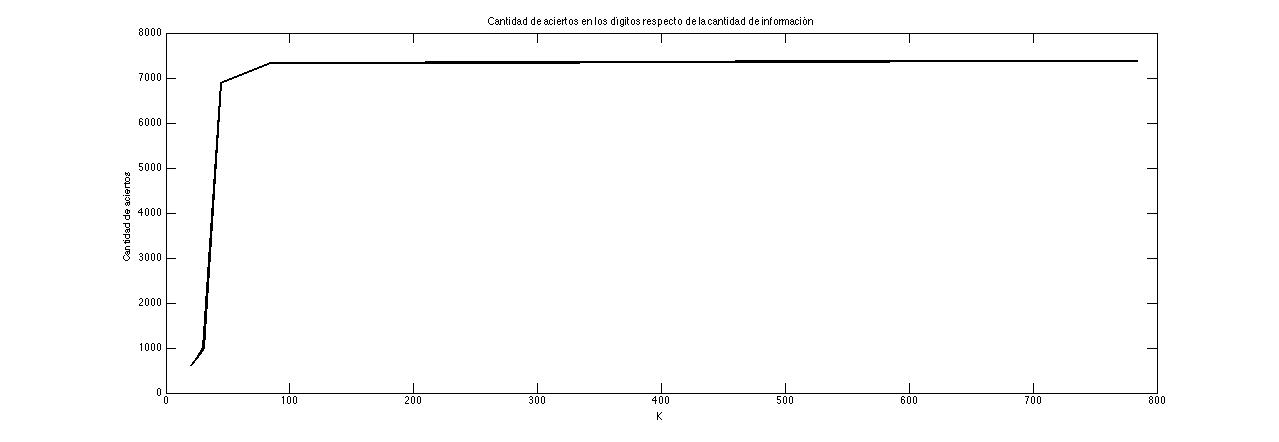
\includegraphics[width=520pt]{./aciertosconk.jpg}
\caption[h]{Cantidad de Aciertos respecto de K a partir de 10000 imágenes.}
\end{center}
\end{figure}

En el gráfico anterior puede observarse que, si bien los resultados son más precisos, alcanza con guardar el 6\% de los datos de cada imagen para alcanzar un 70\% de correctitud en la deducción de caracteres. Esto nos da lugar a pensar que, a pesar de ser mejor lograr una precisión del 73\%, no es realmente necesario almacenar toda la transformada característica de cada dígito para deducirlo. De esta manera, se evita ocupar memoria de manera excesiva y se logra mejorar el tiempo de ejecución de los programas encargados de realizar dichas comparaciones facilitando el reconocimiento de dígitos.

\section{Discusi\'on}
Una vez obtenidos los resultados presentados previamente, nos realizamos cuestionamientos que nos parecieron interesantes para analizar. En primer lugar, pensamos qué podría haber pasado si en vez de realizar el promedio de cada dígito dentro de la base de datos hubiéramos comparado uno a uno con el dígito a determinar. Creemos que los resultados hubieran dependido básicamente de la cantidad de datos mal taggeados. Esto se debe a que la comparación entre la transformada de la imagen a determinar y la transformada de una imagen perteneciente a la base de datos puede resultar muy similar pero el resultante será siempre el de la etiqueta de dicha imagen. El inconveniente que pudo haberse presentado por dígitos mal taggeados fue la probabilidad de que el promedio de éstos fuera desplazado de su centro. Sin embargo, al saber que la mayoría se encuentra correctamente etiquetado, supimos que no afectaría a gran escala los resultados. Por otra parte, si existiese la posibilidad de obtener una base de datos sin problemas de etiquetamiento, pensamos que la comparación con cada elemento de la base de datos daría mejores resultados en la mayoría de los casos (siempre que la cantidad de outliers no fuera demasiado grande). Esto se debe a que la comparación resultaría más exacta y la probabilidad de equivocarse se reduciría enormemente. Del mismo modo, se evitaría correr el riesgo de que dos promedios resulten altamente semejantes por tener representaciones parecidas dando lugar a errores en muchos de sus dígitos (como por ejemplo nuestro caso con los dígitos 4 y 9).\newline
\newline
Por otra parte, pensamos que si no hubiese habido autovalores repetidos, probablemente el Método de Potencia hubiese sido más eficiente que el Método QR pues la cantidad de operaciones y de ciclos a realizar son mucho menores, disminuyendo enormemente el tiempo de ejecución del programa.

\section{Conclusiones}
Luego de las experimentaciones mencionadas anteriormente, pudimos extraer ciertas conclusiones. En primer lugar, podemos afirmar que cuanto mayor es la cantidad de datos en la transformada característica ($X_{i}*V^t$) de cada imagen utilizada para compararlas entre sí con el fin de reconocer el dígito de una de ellas, más preciso es el resultado obtenido pues más límpida resulta la transformada característica de cada dígito. Esto se debe a que cuanto mayor es la cantidad de información, mayor precisión se obtiene.\newline
Por otro lado, pudimos concluir que el Método de Potencia es más simple y claro que el Método QR pero la falta de certeza sobre su convergencia puede aportar grandes problemas a tal punto de dejarlo inutilizable en muchos casos.\newline
Por otra parte, pudimos observar que no es esencial utilizar 60000 datos para realizar reconocimiento de dígitos manuscritos, sino que 10000 imágenes nos alcanzaron perfectamente para obtener muy buenos resultados evitando demorar demasiado el tiempo de ejecución de los mismos.\newline
Por último, podemos afirmar que la utilización de SVD es muy efectiva para el reconocimiento de dígitos, superando ampliamente nuestras espectativas sobre los resultados que esperábamos obtener.

\section{Ap\'endices}
\subsection{A}

\begin{centering}
\large\bf Laboratorio de M\'etodos Num\'ericos - Primer Cuatrimestre 2013 \\
\large\bf Trabajo Pr\'actico N\'umero 3: OCR+SVD\\
\end{centering}


\vskip 0.5 cm
\hrule
\vskip 0.1 cm

{\bf Introducci\'on}

El reconocimiento \'optico de caracteres (OCR, por sus siglas en ingl\'es) es el proceso por el cual se traducen o convierten im\'agenes de d\'igitos o caracteres (sean \'estos manuscritos o de alguna tipograf\'ia especial) a un formato representable en nuestra computadora (por ejemplo, ASCII). Esta tarea puede ser m\'as sencilla (por ejemplo, cuando tratamos de determinar el texto escrito en una versi\'on escaneada a buena resoluci\'on de un libro) o tornarse casi imposible (recetas indescifrables de m\'edicos, algunos parciales manuscritos de alumnos de m\'etodos num\'ericos, etc).

El objetivo del trabajo pr\'actico es implementar un m\'etodo de reconocimiento de d\'igitos manuscritos basado en la descomposici\'on en valores singulares, y analizar emp\'iricamente los par\'ametros principales del m\'etodo.

Como instancias de entrenamiento, se tiene un conjunto de $n$ im\'agenes de d\'igitos ma\-nus\-cri\-tos en escala de grises del mismo tama\~no y resoluci\'on (varias im\'agenes de cada d\'igito). Cada una de estas im\'agenes sabemos a qu\'e d\'igito se corresponde.
En este trabajo consideraremos la popular base de datos MNIST, utilizada como referencia en esta \'area de investigaci\'on\footnote{\texttt{http://yann.lecun.com/exdb/mnist/}}. 

Para $i = 1,\ldots, n$, sea $x_i \in \real^{m}$ la $i$-\'esima imagen de nuestra base de datos almacenada por filas en un vector, y sea $\mu = (x_1 + \ldots + x_n)/n$ el promedio de las im\'agenes. Definimos $X\in\real^{n\times m}$ como la matriz que contiene en la $i$-\'esima fila al vector $(x_i - \mu)^{t}/\sqrt{n-1}$, y $$X=U \Sigma V^t$$ a su descomposici\'on en valores singulares, con $U\in\real^{n\times n}$ y $V\in\real^{m\times m}$ matrices ortogonales, y $\Sigma\in\real^{n\times m}$ la matriz diagonal conteniendo en la posici\'on $(i,i)$ al $i$-\'esimo valor singular $\sigma_i$.
Siendo $v_i$ la columna $i$ de $V$, definimos para $i = 1,\ldots,n$ la \textsl{transformaci\'on caracter\'istica} del d\'igito $x_{i}$ como el vector $\mathbf{tc}(x_i) = (v_1^t\, x_i, v_2^t\, x_i,\ldots,v_k^t\, x_i) \in\real^k$, donde $k \in\{1,\ldots,m\}$ es un par\'ametro de la implementaci\'on. Este proceso corresponde a extraer las $k$ primeras \textit{componentes principales} de cada imagen. La intenci\'on es que $\mathbf{tc}(x_i)$ resuma la informaci\'on m\'as relevante de la imagen, descartando los detalles o las zonas que no aportan rasgos distintivos.


Dada una nueva imagen $x$ de un d\'igito manuscrito, que no se encuentra en el conjunto inicial de im\'agenes de entrenamiento, el problema de reconocimiento consiste en determinar a qu\'e d\'igito corresponde. Para esto, se calcula $\mathbf{tc}(x)$ y se compara con $\mathbf{tc}(x_i)$, para $i = 1,\ldots, n$.


{\bf Enunciado}

Se pide implementar un programa que lea desde archivos las im\'agenes de entrenamiento de distintos d\'igitos manuscritos y que, utilizando la descomposici\'on en valores singulares, se calcule la transformaci\'on caracter\'istica de acuerdo con la descripci\'on anterior. Para ello se deber\'a implementar alg\'un m\'etodo de estimaci\'on de autovalores/autovectores. Dada una nueva imagen de un d\'igito manuscrito, el programa deber\'a determinar a qu\'e d\'igito co\-rres\-pon\-de.
El formato de los archivos de entrada y salida queda a elecci\'on del grupo. Si no usan un entorno de desarrollo que incluya bibliotecas para la lectura de archivos de im\'agenes, sugerimos que utilicen im\'agenes en formato \textsc{Raw}. 


Se deber\'an realizar experimentos para medir la efectividad del reconocimiento, analizando tanto la influencia de la cantidad $k$ de componentes principales seleccionadas como la influencia de la precisi\'on en el c\'alculo de los autovalores.

\vskip 0.5 cm
\hrule
\vskip 0.1 cm

{\bf Fecha de entrega} 
\begin{itemize}
\item \textsl{Formato electr\'onico:} viernes 21 de junio de 2013, \underline{hasta las 23:59 hs.}, enviando el trabajo (informe+c\'odigo) a \texttt{metnum.lab@gmail.com}. El subject del email debe comenzar con el texto \verb|[TP3]| seguido de la lista de apellidos de los integrantes del grupo. 
\item \textsl{Formato f\'isico:} lunes 24 de junio de 2013, de 18 a 20hs (en la clase de la pr\'actica).
\end{itemize}

\subsection{B}

\large{\textbf{Implementaci\'on de nuestro programa:}}\newline

\centerline{\large{\textbf{Matriz.cpp}}}

\lstloadlanguages{C++}
\lstset{language=C++,texcl=true,inputencoding=utf8/latin1,showstringspaces=false,
	frame=Ltb,
     framerule=0pt,
     aboveskip=0.5cm,
     framextopmargin=3pt,
     framexbottommargin=3pt,
     framexleftmargin=0.4cm,
     rulesep=.4pt,
    framesep=5pt,
basicstyle=\normalsize\ttfamily,
showstringspaces=false,
keywordstyle=\color{blue},
%identifierstyle=\ttfamily,
stringstyle=\color{Maroon},
commentstyle=\color{black},
rulecolor=\color{Gray},
xleftmargin=5pt,
xrightmargin=5pt,
aboveskip=\bigskipamount,
belowskip=\bigskipamount,
}
\lstinputlisting[language=C++]{Matriz.cpp}

\centerline{\large{\textbf{Matriz.h}}}
\lstinputlisting[language=C++]{Matriz.h}

\centerline{\large{\textbf{main.cpp}}}
\lstinputlisting[language=C++]{main.cpp}

\section{Referencias}

%%un libro se referencia asi AUTOR. Año. Título; subtítulo. Edición. Lugar de publicación, editorial. Páginas o
%%volumen. (Serie comercial)

\begin{itemize}

\item BURDEN, RICHARD L. ; An\'alisis num\'erico, 7ma ed. 2002. M\'exico, Thomson Learning.

\item http://definicion.de/
\item http://www.iti.es/media/about/docs/tic/13/articulo2.pdf
\item http://mathworld.wolfram.com/Covariance.html
\item http://yann.lecun.com/exdb/mnist/

\end{itemize}

\end{document}
